\chapter{TenderInsights}

\section{Kurze Projektbeschreibung}
In dem Projekt geht es darum einen PoC - also einen Proof of Concept zu erstellen, der mithilfe von AI bzw. Large
Language Models (LLM) große Dokumente nach gesuchten Inhalten durchsucht und aufbereitet. Im Fokus stehen dabei
insbesondere öffentliche Ausschreibungen zur Akquise von neuen Projekten für das Unternehmen. Bisher hat ein Mitarbeiter
aus PMO die Ausschreibungen händisch grob für passend oder nicht geeignet erklärt und dann an die Akquise
weitergeleitet. Dort hat ein Mitarbeiter die Ausschreibung sehr genau analysiert und einen sogenannten One Pager
erstellt, der alle Daten welche für eine Entscheidung, ob man sich bewerben möchte oder nicht, relevant sind. Aufgabe
des PoC ist es nun diesen One Pager mithilfe von künstlicher Intelligenz und einem LLM aus einer oder mehreren
bereitgestellten PDF-Datei zu generieren. Der Anwender soll dies über ein Userinterface im Stile einer Webanwendung
bedienen können.

\section{Verwendete Software und Grundlagen}
In diesem Kapitel werden alle Technologien und Begriffe beschrieben, welche im Entwicklungsumfeld des TenderInsights
verwendet werden oder für ein Verständnis zuträglich sind.

\subsection{Technologien}
Bei der Entwicklung des TenderInsights werden viele unterschiedliche Technologien eingesetzt. Während meines Praktikums
habe ich in meiner Tätigkeit als Entwickler viele davon kennengelernt und verwendet. Nachfolgend erkläre ich die
wichtigsten Technologien.

\subsubsection{Python}
Python ist eine höhere Programmiersprache welche sich durch ihre klare und leicht verständliche Syntax auszeichnet. Sie
ist bekannt für ihre zahlreichen Standardbibliotheken und ihrer reichen Auswahl an Modulen und Frameworks. Da OpenAI nur
JavaScript und Python unterstützt, und Python aus zuvor genannten Gründen einsteigefreundlicher ist wurde sich für diese
Sprache entschieden.

\subsubsection{Langchain}
Langchain ist ein Open-Source-Framework, das auf die Entwicklung und integration von Sprach-KI-Anwendungen spezialisiert
ist. Es erleichtert das einbinden von Sprachmodellen wie GPT-3.5-turbo von openAI in Projekte und wird beim
TenderInsights für Textgenerierung verwendet.

\subsubsection{OpenAI - GPT}
OpenAI ist ein US-Amerikanisches Unternehmen welches sich mit der Erforschung und Entwicklung von künstlicher
Intelligenz beschäftigt. Eines der bekanntesten Tools bzw. Frameworks ist GPT - Generative Pretrained Transformer, ein
Sprachverarbeitungsmodell zur Textgenerierung, Übersetzung, Zusammenfassung und mehr. GPT wird im TenderInsights
verwendet um Information aus Texten zu extrahieren und um die gelieferten Prompts zu bewerten.

\subsubsection{Azure}
Microsoft Azure ist eine Cloud-Computing-Plattform, welche eine breite Palette von Diensten und Lösungen für Unternehmen
und Entwickler bietet. Zu den Entwickler-Tools und -Diensten gehört unter anderem Azure openAI, welches eine openAI API
zur Verfügung stellt. Im Gegensatz zu openAI befinden sich die Server in Europa, weshalb im späteren Verlauf des
Projekts aus Gründen des Datenschutzes zu Azure gewechselt wurde.

\subsubsection{ChromaDB}
ChromaDB ist eine Open-Source-Datenbanklösung, welche speziell für die Arbeit mit Vektor-Einbettungen in KI-Anwendungen
entwickelt wurde. Da der Kontext für Sprachmodelle stark unter der Größe von durchschnittlichen Dokumenten liegt wird
eine Vektor-Datenbank genutzt um die relevanten Stellen in den Dokumenten zu finden und als Kontext mit dem Prompt an
das Sprachmodell für die Textgenerierung zu übergeben.

\subsubsection{JSON}
JavaScript Object Notation, oder kurz JSON, ist ein Daten-Austauschformat welches häufig verendet wird um Daten zwischen
einem Server und einer Webanwendung zu übertragen. Da es für Menschen gut lesbar und für Maschinen einfach zu parsen
(Entspricht einem normalen Dictionary in Python) ist eignet es sich hervorragend für das Speichern der OnePager
Informationen.

\subsection{Wichtige Begriffe}

\begin{table}[H]
    \centering
    \caption{Wichtige Begriffe}
    \label{tab:technologien}
    \begin{tabular}{|>{\centering\arraybackslash}m{4cm}|p{10cm}|} % Anpassen der Breitenangaben nach Bedarf
    \hline
    \textbf{Name} & \textbf{Beschreibung} \\ \hline
    Prompt & Anleitung oder Frage die dem Sprachmodell vorgibt, was es tun soll. Auch Eingabeaufforderung genannt. \\ \hline
    Prompt Engineering & Gestalten und Optimieren von Eingabeaufforderungen (Prompts) \\ \hline
    Token & Grundlegender Baustein für die Verarbeitung und das Verständnis von Sprache in KI-Systemen  \\ \hline
    Embedding & Einbetten von Text in Vektoren \\ \hline
    Vektordatenbank & Datenbank welche die aus dem Embedding generierten Vektoren enthält \\ \hline
    Similarity Search & Suche von nahestehenden Vektoren innerhalb der Vektordatenbank um gesuchte Dokumenteninhalte zu
    finden \\ \hline
    Large Language Model (LLM) & Fortgeschrittene KI, die umfangreiche Textdaten versteht und generiert, basierend auf umfassendem Training und komplexen Algorithmen \\ \hline
    \end{tabular}
\end{table}

\section{Projektstand bei Arbeitsbeginn}
Zum Zeitpunkt meines Projekteintrittes gibt es bereits ein Frontend welches mithilfe von Streamlit implementiert wurde. 
PDF-Dateien können über einen File-Uploader im Frontend an die Anwendung übergeben werden. Da die meisten LLM-Modelle eine 
begrenzte Token-Anzahl für die Abfragen haben ist es nicht möglich das gesamte Dokument an das LLM zu übergeben. 
Daher wird das Dokument aufgesplittet und mittels einer Vektordatenbank auf Ähnlichkeit mit die gesuchte Information 
abgeglichen. Die k Ergebnisse mit der größten Ähnlichkeit werden zusammen mit dem Prompt als Abfrage an das LLM übermittelt. 
Die Abfragen werden mit der Langchain API durchgführt, das verwendete Modell ist "gpt-3.5 turbo". Es gibt 3 Ausschreibungsdokumente 
in verschiedenen Größen mit denen die Abfragen getestet werden können. Es gibt 3 Prompts, welche bislang nur bedingt gute 
Ergebnisse liefern.

\section{Softwarearchitektur der Anwendung zum Zeitpunkt der BUILD23}
Um nachfolgende Kapitel besser verstehen zu können erkläre ich in diesem Kapitel die Grobe Software-Architektur der
Anwendung zum Zeitpunkt der BUILD23 anhand der Abbildung \ref{fig:DokumentenAgent-uebersicht}.

\begin{figure}[h]
    \centering
    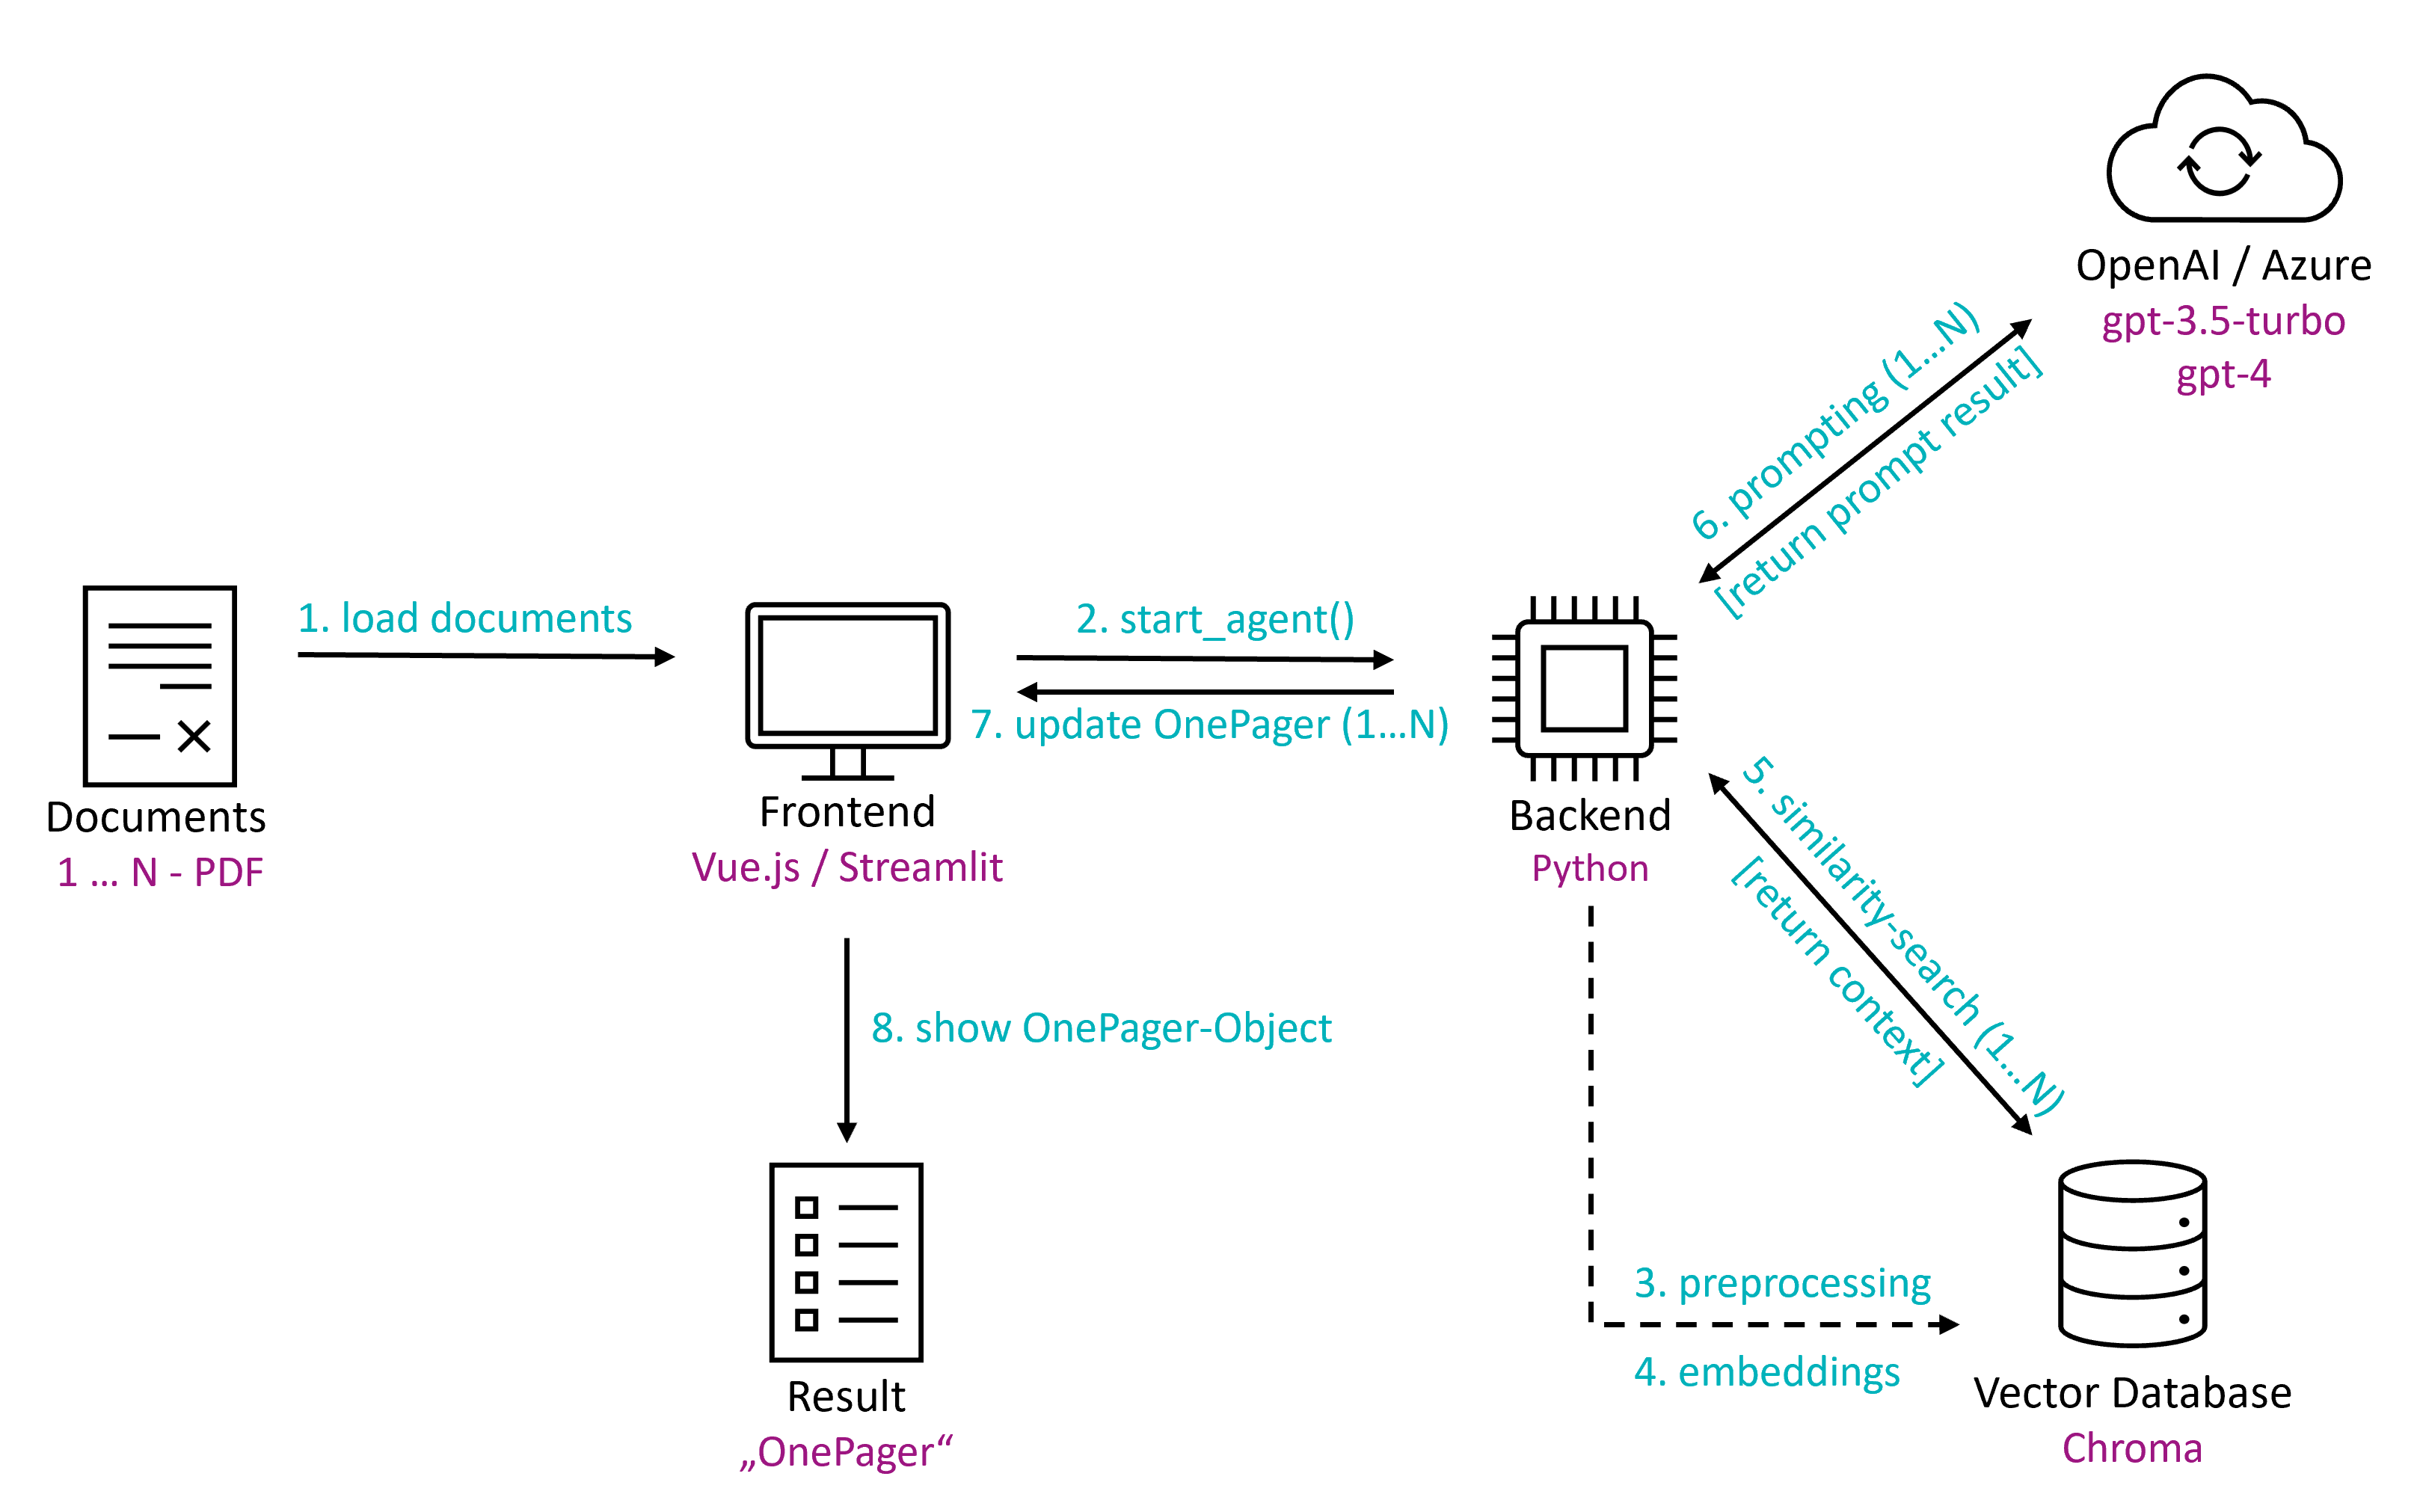
\includegraphics[width=0.8\textwidth]{figures/DokumentenAgent-Uebersicht.png}
    \caption{Schematische Darstellung der Software-Architektur}
    \label{fig:DokumentenAgent-uebersicht}    % \ref{fig:DokumentenAgent-uebersich}
\end{figure}

Zuerst werden die Ausschreibungsdokumente im Frontend hochgeladen (Siehe 1.) und der Agent wird mit den gewünschten Prompts
gestartet (Siehe 2.). Der Agent beginnt nun im Backend mit dem PreProcessing, welches die Dokumente in fachlich logische Blöcke
aufspaltet und personenbezogene Daten anonymisiert (Siehe 3.). Anschließend wird das Embedding, also eine Repräsentation der Daten
als Vektoren, erstellt und als der Vektordatenbank angelegt (Siehe 4.). Nun wird für jeden Prompt eine Similarity-Search
durchgeführt (Siehe 5.), bei der dem möglichst passende Stellen aus den Dokumenten aus der Vektordatenbank extrahiert werden, damit
diese im Prompt als Kontext eingebettet für die Textvervollständigung an das LLM übergeben werden (Siehe 6.). Das Ergebnis wird in
ein JSON-Objekt übersetzt und der OnePager wird entsprechend aktualisiert (Siehe 7.). Währenddessen baut sich im Frontend Stück für
Stück der OnePager mit allen gefundenen Informationen zusammen (Siehe 8.).

\section{Meine Rolle und Aufgaben im Projekt}
Ich bin in der Rolle eines Softwareentwickler in das Projekt gekommen. Meine Aufgabe bestand Anfangs darin, die Prompts für die einzelnen 
Felder des One Pagers zu formulieren um die gelieferten Ergebnisse zu verbessern. Dies resultierte in den Aufbau einer 
Test- und Evaluierungsarchitektur in Python mithilfe derer die Prompts vollautomatisch bewertet werden und anhand ihrer Kennzahl 
ausgewählt und weiter optimiert werden. Durch Komplikationen mit dem Datenschutz wurde der Umstieg von Langchain auf 
Azure von Microsoft beschlossen, welchen ich durchgeführt habe. 

\subsection{Prompt Engineering}
Um gute Ergebnisse durch die Textvervollständigung der Sprachmodelle zu erhalten ist es unumgänglich hochwertige Prompts zu formulieren.
Hierfür habe ich mehrere E-Learnings zum Thema Prompt Engineering absolviert, in denen erklärt wird wie man hochwertige Prompts erstellt und 
ganze Systeme mit einer Chatbotintegration entwickelt. Besondere Methoden welche im Projekt zum Einsatz kommen sind Single-Shot-Prompting, 
bei dem man ein Beispiel gibt wie eine optimale Antwort auszusehen hat, und die Ausgabe als JSON festzulegen, um die erhaltenen Ergebnisse 
im Code nutzen und anwenden zu können. Das Abgrenzen von wichtigen Informationen wie dem mitgelieferten Kontext über sogenannte Delimiter hilft
dem Modell dabei, Aufgabe und Kontext nicht zu vermischen (wenn auch nicht immer perfekt). Gut eignet sich hierfür '\#\#\#\#', da dies als 
ein Token zählt und selten regulär vorkommt. Um Halluzinationen, also das produzieren von Falschinformationen oder ausgedachten Informationen zu 
vermeiden wird im Prompt explizit darauf hingewiesen, dass bei nicht vorhandenen Informationen das entsprechende Feld leer gelassen werden soll. 
%Das Bewerten der generierten Antworten durch das Sprachmodell um die Qualität zu messen, welches später im Kapitel \ref{chap:Evaluation} Verwendung findet.

\subsection{OnePager}
Der von PMO erstellte OnePager umfasst alle wesentlichen Information der Ausschreibung um eine fundierte Entscheidung darüber treffen zu 
können, ob die Ausschreibung als Projekt für iteratec geeignet ist. Informationen sind unter anderem der Projekttitel, eine kurze Projektbeschreibung, 
Adressdaten über das Ausschreibende Unternehmen oder Amt, wichtige Termine und Deadlines, Bewertungskriterien, Aufgaben und benötigte Unterlagen welche 
dem Angebot beigefügt werden müssen. Da jede dieser Punkte in unterschiedlichen Regionen der Dokumente zu finden ist und die Qualität der Ergebnisse 
besser ist wenn man nicht mehrere Fragen in einer Anfrage bündelt wird der OnePager in der Anwendung Frage für Frage zusammengesetzt und ergänzt.
Als Format wird JSON verwendet um später den fertigen OnePager gut speichern und weiterverarbeiten zu können (zum Beispiel für die Evaluation) und um dem
Frontend die Daten als Variable zur Verfügung zu stellen. Die OnePager-Klasse wurde wurde um viele Hilfsmethoden ausgestattet um das Arbeiten mit den 
JSON-Objekten zu erleichtert. Zu den Hilfsmethoden gehören unter anderem das initialisieren des OnePager-Template, das laden und abspeichern als Datei, 
einfaches hinzufügen von Teilinformationen aus den einzelnen Ergebnissen des Sprachmodells in den bestehenden OnePager und Prüffunktionen um nicht 
JSON-Konforme Antworten zu erkennen.

\subsection{Verbessern der Kontextauswahl über Similarity Search}
\label{chap:Verbessern der Kontextauswahl über Similarity Search}
Um gezielt die fachlich richtigen Passagen innerhalb des Dokuments zu finden wird eine query gegen die über das
Embedding generierte Vektordatenbank gestellt. Als Ergebnis erhält man die n-Textausschnitte, mit der höchsten
Trefferquote. Bei dem eben beschriebenen Verfahren sprechen wir von einer Similarity Search, also dem finden von
ähnlichen Daten innerhalb einer Vektorrepräsentation des bereitgestellten Dokuments. Da es bei Ausschreibungen viele
synonyme Begriffe gibt, welche Informationen zu identischen Fragestellungen geben habe ich diese Begriffe in einem
Lexikon erfasst und gesammelt. Die Akquiseabteilung wurde zusätzlich darum gebeten weitere Ergänzungen vorzunehmen um
fachlich möglichst viele Begriffe abzudecken. Mit dem so erhaltenen Lexikon können wichtige Keywords für die Similarity
Search bereitgestellt werden, vereinzelt wird auch innerhalb der Prompts darauf zurückgegriffen um das Sprachmodell
dabei zu unterstützen die richtigen Informationen der richtigen Stelle des OnePagers zuzuordnen. Über ein Prompt.Config
Dictionary kann nun für jedes Prompt auf entsprechende Felder wie Suchbegriffe, Promptmethode oder Suchergebnisanzahl
individuell zugegriffen werden.

\subsection{Evaluation} 
\label{chap:Evaluation}   
Um festzustellen ob sich Prompts beim Wechsel von Modellen, Promptversionen oder unterschiedlichen PreProcessing-Verfahren verbessern oder verschlechtern 
habe ich 10 Testdatensätze aus öffentlichen Ausschreibungsportalen zusammmengesucht und entsprechende Musterlösungen erarbeitet, sofern dies in unserem 
fachlichen Rahmen möglich war. Dies hat uns ermöglicht, ausgewählte Prompts testweise gegen alle 10 Testdatensätze abzufragen. Hierbei wird die neu 
generierte Antwort mit der Musterlösung verglichen und anschließend anhand eines Bewertungsschemas mit Punkten zwischen 0 und 10 inklusive einer 
Begründung bewertet, je nachdem wie nah das gelieferte Ergebnis an die Musterlösung herankommt.    

\begin{figure}[h]
    \centering
    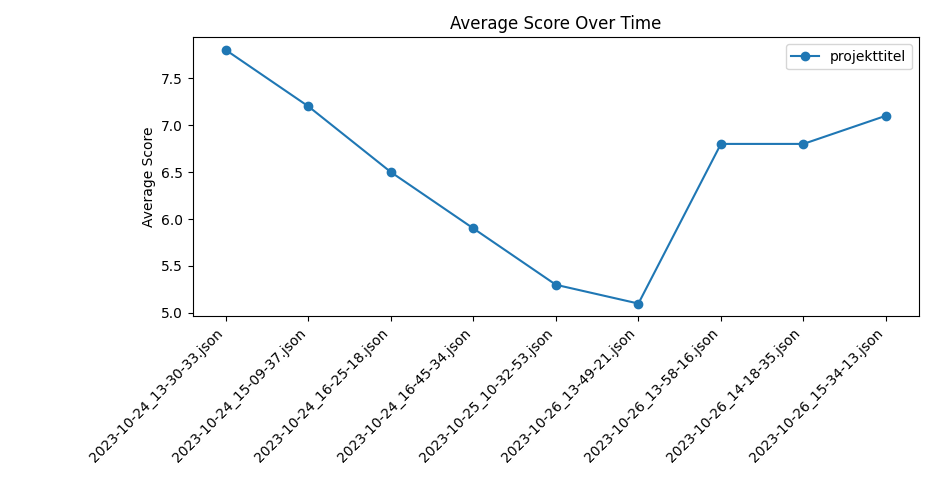
\includegraphics[width=0.8\textwidth]{figures/02_Prompt_Evaluierung.png}
    \caption{Visualisierung eines Prompts mit verschiedenen Prompt und Bewertungsmodifikationen über Zeit}
    \label{figure:02_Prompt_Evaluierung}     % \ref{figure:02_Prompt_Evaluierung}
\end{figure}

Die einzelnen Punkte werden anschließend für jedes Prompt zu einem Average Score zusammengerechnet und mithilfe der Visualisierungsklasse als Plot dargestellt. 
Dabei können einzelne Prompts über verschiedene Versionen und Zeitpunkte (siehe \ref{figure:02_Prompt_Evaluierung}) oder mehrere Prompts bei Verwendung 
unterschiedlicher Sprachmodelle (siehe \ref{fig:04_Prompt_Evaluierung-MitPreProcessing}) dargestellt und verglichen werden.

\begin{figure}[h]
    \centering
    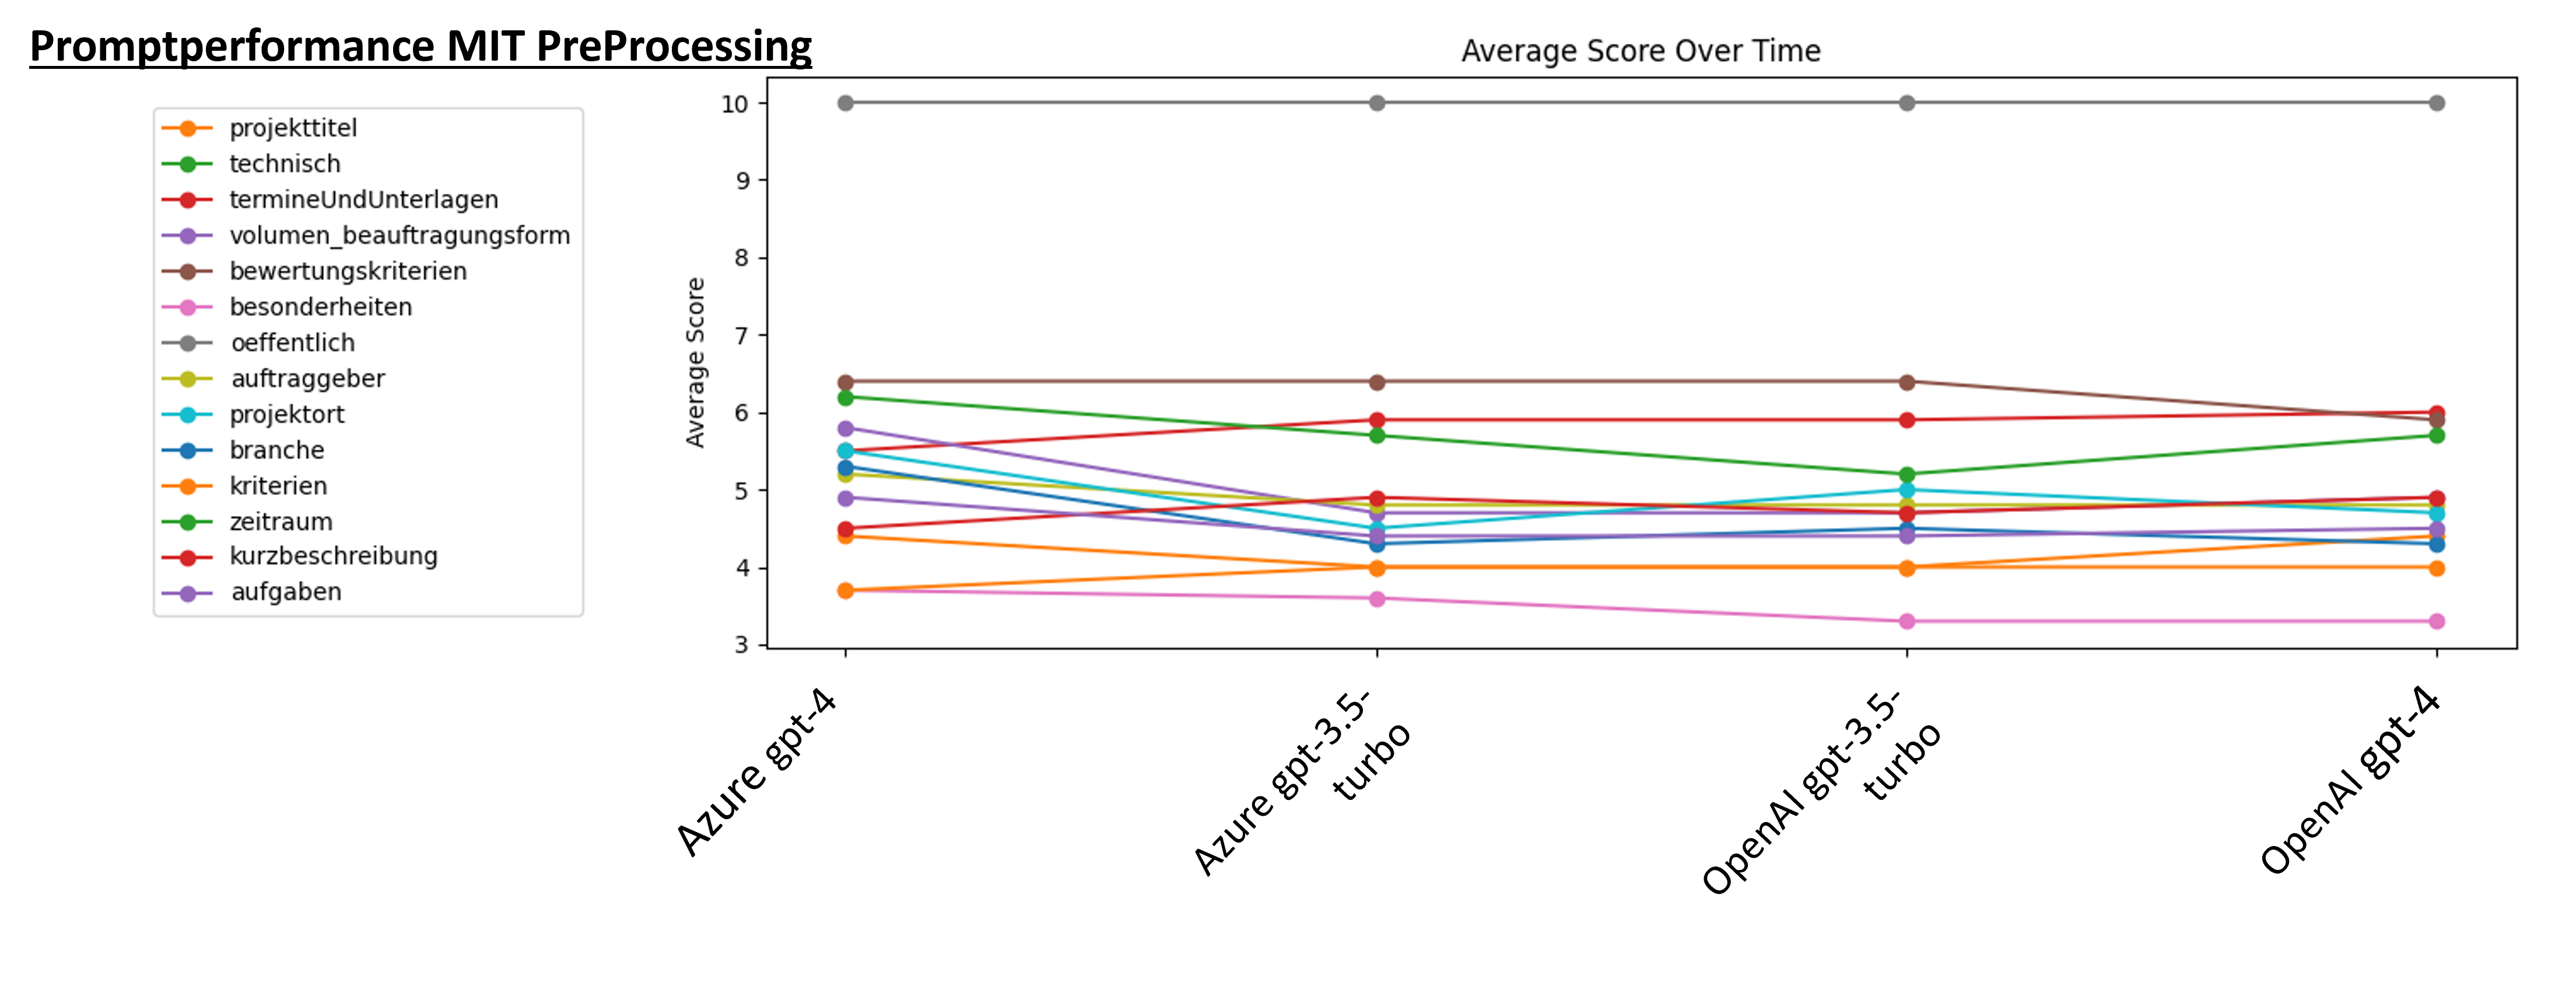
\includegraphics[width=0.8\textwidth]{figures/04_Prompt_Evaluierung-MitPreProcessing.png}
    \caption{Visualisierung der Prompts mithilfe unterschiedlicher Modelle. PreProcessing ist aktiviert}
    \label{fig:04_Prompt_Evaluierung-MitPreProcessing}    % \ref{fig:04_Prompt_Evaluierung-MitPreProcessing}
\end{figure}

\subsection{Azure Migration}
Da die rechtliche Lage bei der Verarbeitung Personenbezogener Daten durch Sprachmodelle wie gpt laut unserer
Datenschutzbeauftragten noch sehr unklar ist bis es erste Urteile geben wird, wurde sich darauf geeinigt auf azure
openAI zu migrieren da dort europäische Server verwendet werden statt amerikanischer. Ein großer Nachteil von Azure ist
aber, dass man für das erstellen der Embeddings für die Vektordatenbank auf 16 Inputs beschränkt ist, während openAI
hier keine Einschränkungen vorgibt. Größere Dokumente können leicht auf 1 Input pro Seite kommen, was ein Einbetten von
Dokumenten ab 20 Seiten verhindert. Um das Problem zu lösen habe ich statt die vorgegebene Embedding-Methode zu
verwenden eine eigene Methode erstellt, welche die Dokumente bzw. die Inputs auf mehrere Listen mit einer Größe kleiner
gleich 16 aufteilt. Anschließend werden die einzelnen Listen über eine REST API zu embeddings umgewandelt und wieder
zusammengesetzt. Am ende wird eine Collection mit den Embeddings, den Dokumenten und entsprechenden Metadaten erstellt,
welche zentral in einem VectorDataManager zur Verfügung gestellt wird. Gegen diese Collection können anschließend
Abfragen wie Similarity-Searches (siehe \ref{chap:Verbessern der Kontextauswahl über Similarity Search}) durchgeführt
werden. 

\subsection{Dokumentation}
Sämtlicher von mir geschriebener Quellcode wurde mit Ein- und Mehrzeiligen Kommentaren ergänzt, um das Lesen und
Verstehen des Codes zu vereinfachen. Ich habe die gesammelten Erfahrungen in einem Bericht festgehalten und diesen im
Repository abgelegt. Zudem wurden Architecture Decision Records, kurz ADR, erstellt und ebenfalls dem Projekt angehängt.
Diese ADRs sind dazu da, später Einsicht darüber zu geben warum sich für bzw. gegen ein Framework oder eine Technologie 
entschieden wurde. 

\subsection{Messestand auf der BUILD23}

Zum Abschluss des Projektes wurden wir angefragt, ob wir 
aufgrund des hohen Interesses an dem Projekt eine Präsentation während des GS-Meetings und der BUILD23 halten möchten. 
Das erstellen der Präsentation und Vortragen dieser gehörte auch zu meinem Aufgabenbereich.


\section{Herausforderungen und Lösungsansätze}

\subsection{Optimierung der Prompts}
Um die Prompts zu verbessern ist es notwendig, diese an unterschiedlichen Ausschreibungen zu testen und das gelieferte 
Ergebnis mit der richtigen Antwort zu vergleichen. Da das größte Dokument über 100 Seiten hat und wir keine Musterlösungen 
haben war es schwierig Aussagen über die Qualität der Prompts zu treffen. Die Lösung war das Einführen einer Metrik welche 
die Qualität der Prompts misst. Es wurden 10 Dokumente ausgearbeitet und sämtliche wichtige Informationen in OnePager-JSON Dateien 
gespeichert. Anschließend wurde eine Testarchitektur geschaffen, in welcher man die gewünschten Prompts vollautomatisiert 
gegen die 10 Testdokumente abfragt und anschließend die Resultate zusammen mit der Musterlösung von ChatGPT auf inhaltliche 
Übereinstimmung überprüfen und bewerten lässt.

[SIEHE ANHANG XXX - Evaluationsprompt]

Aus den so generierten Bewertungen lassen sich nun Aussagekräftige Kennzahlen 
generieren. Zur Darstellung wurde eine Visualisierungsklasse geschrieben, welche die Punktzahl der Prompts graphisch darstellt 
(siehe \ref{fig:03_Prompt_Evaluierung}) und so schnell erkennbar ist, ob der aktuelle Prompt zu einer Verbesserung 
oder Verschlechterung der Ergebnisse führt.

\begin{figure}[H]
    \centering
    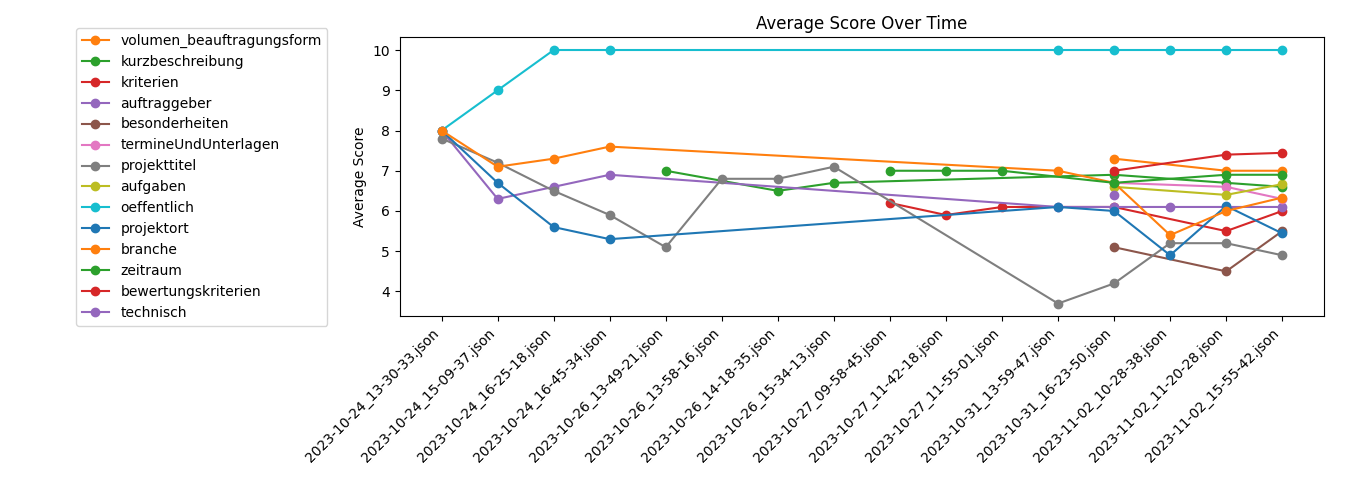
\includegraphics[width=0.8\textwidth]{figures/03_Prompt_Evaluierung.png}
    \caption{Visualisierung der durchschnittlichen Promptqualität im Laufe der Zeit}
    \label{fig:03_Prompt_Evaluierung}    % \ref{fig:03_Prompt_Evaluierung}
\end{figure}

\subsection{Datenschutz}
Das übermitteln und verarbeiten von Personenbezogenen Daten ist in Deutschland nur mit Ausdrücklicher Genehmigung der
entsprechenden Person zulässig. Laut unserer Datenschutzbeauftragten ist unklar inwiefern das Übermitteln der Daten aus
den Dokumenten über die OpenAI API hierunter einzustufen ist. Offiziell heißt es, dass die Daten, welche über die API
geteilt werden, nicht zu Trainingszwecken genutzt werden. Da die Server von OpenAI allerdings in den USA liegen
gestalten sich Probleme mit europäischen Datenschutzrecht. Als Lösung wurde die Umstellung auf Azure in Betracht
gezogen, da die Server auf europäischen Boden stehen und damit zumindest nach europäischen Recht Datenschutzkonform
sind. Zusätzlich anonymisieren wir so gut wie alle Personenbezogenen Daten bevor wir diese an das Sprachmodell
übermitteln, indem wir den Kontext vor dem Abschicken gegen eine Liste an Namen prüfen, und so Namen und Mailadressen
herausfiltern.

\section{Ergebnisse und Erfahrungen}

\subsection{Proof of Concept}
Aus den gesammelten Ergebnissen und Erfahrungen lässt sich herleiten, dass der PoC definitiv zeigt, dass die Anwendung
so möglich ist. Auch wenn nicht immer alle OnePager korrekt generiert wurden, und teils immer noch Halluzinationen
vorkommen und wichtige Informationen fehlen so funktioniert die Anwendung im Kern so wie sie es soll. Wichtig für die
Zukunft ist es Klarheit beim Umgang mit Personenbezogenen Daten im Zusammenhang mit Sprachmodellen zu schaffen und
gegebenenfalls eine geeignete Filterung dieser Daten zu implementieren. Durch neue Modelle, wie dem gegen Ende des
Projekts angekündigten gpt-4-turbo, welches eine Kontextlänge von 128K Tokens besitzt, wird man nicht länger gezwungen
sein sich auf kleine Textausschnitte zu begrenzen. Man kann ganze Kapitel übergeben und Limitierungen haben mehr
wirtschaftliche Gründe als Technische. Auch die Fehleranfälligkeit wird durch einen eingebauten JSON-Parser weiter
sinken. Unsere Tests zeigen keine Nennenswerte Unterschiede zwischen den Modellen gpt-3.5-turbo und gpt-4 was die
Qualität der Prompts angeht, daher ist es unwahrscheinlich, dass das neue Modell hier tatsächlich einen Unterschied
macht.

\subsection{Persönlich}
Persönlich konnte ich in dem Projekt lernen, wie man mithilfe eines Jira-Boards als Gruppe iterativ Software entwickelt.
Ich habe mit Python eine neue Programmiersprache gelernt, welche vielseitig einsetzbar ist und vor allem im Bereich der
Künstlichen Intelligenz und Machine Learning viele Möglichkeiten bietet. Zudem konnte ich ein tieferes Verständnis für
Prompts und deren Einsatzmöglichkeiten entwickeln. Das entwickeln einer ganze Applikation, welche Sprachmodelle oder
andere LLMs integriert ist für mich nun verständlich und durchführbar. Ich konnte auch Erfahrungen im Dokumentieren von
Entwicklungsartefakten und Entscheidungen sammeln, welche sich in zukünftigen Projekten weiter vertiefen lassen. 